% DeepCNCF architecture diagram.
% Build (from this folder):
%   pdflatex architecture.tex
%   pdftocairo -svg architecture.pdf architecture.svg
\documentclass[tikz,border=6pt]{standalone}
\usepackage[scaled]{helvet}
\renewcommand{\familydefault}{\sfdefault}
\usetikzlibrary{positioning,fit,backgrounds,arrows.meta,calc}

% Palette
\definecolor{dataC}{HTML}{2563EB}
\definecolor{trainC}{HTML}{D97706}
\definecolor{ragC}{HTML}{059669}
\definecolor{ink}{HTML}{1F2937}
\definecolor{muted}{HTML}{6B7280}

\begin{document}
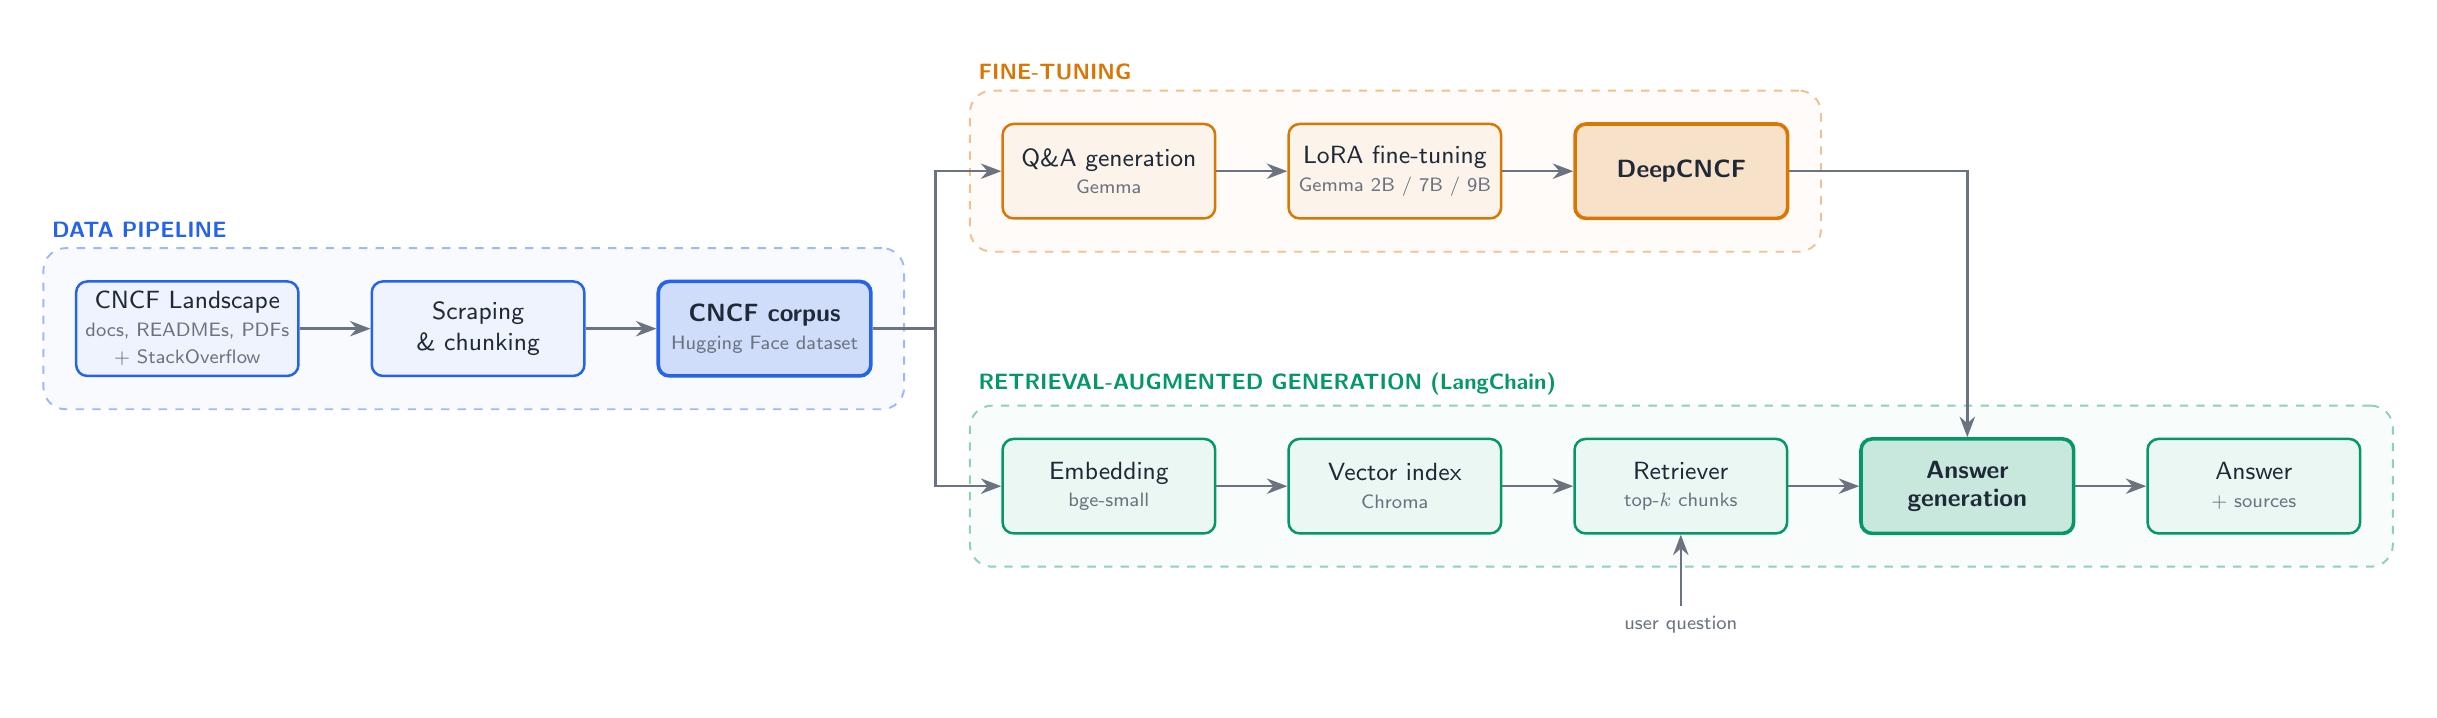
\begin{tikzpicture}[
    font=\small\color{ink},
    node distance=6mm and 9mm,
    box/.style={draw=#1, fill=#1!8, line width=0.9pt, rounded corners=4pt,
                minimum width=27mm, minimum height=12mm, align=center},
    key/.style={box=#1, fill=#1!22, line width=1.3pt, font=\small\bfseries\color{ink}},
    flow/.style={-{Stealth[length=2.6mm]}, line width=0.9pt, draw=muted},
    panel/.style={draw=#1!45, fill=#1!3, rounded corners=8pt, line width=0.7pt,
                  dashed, inner xsep=4mm, inner ysep=4mm},
    title/.style={font=\footnotesize\bfseries\color{#1}, anchor=south west},
    sub/.style={font=\scriptsize\color{muted}},
]

% ---------------- Data pipeline (middle row) ----------------
\node[box=dataC] (src) at (0,0) {CNCF Landscape\\[-1pt]{\scriptsize\color{muted} docs, READMEs, PDFs}\\[-1pt]{\scriptsize\color{muted} + StackOverflow}};
\node[box=dataC, right=of src] (scrape) {Scraping\\\& chunking};
\node[key=dataC, right=of scrape] (corpus) {CNCF corpus\\[-1pt]{\scriptsize\color{muted}\normalfont Hugging Face dataset}};

% ---------------- Fine-tuning (top row) ----------------
\node[box=trainC] (qa) at ($(corpus.east)+(3.0,2.0)$) {Q\&A generation\\[-1pt]{\scriptsize\color{muted} Gemma}};
\node[box=trainC, right=of qa] (ft) {LoRA fine-tuning\\[-1pt]{\scriptsize\color{muted} Gemma 2B / 7B / 9B}};
\node[key=trainC, right=of ft] (model) {DeepCNCF};

% ---------------- RAG (bottom row) ----------------
\node[box=ragC] (emb) at ($(corpus.east)+(3.0,-2.0)$) {Embedding\\[-1pt]{\scriptsize\color{muted} bge-small}};
\node[box=ragC, right=of emb] (index) {Vector index\\[-1pt]{\scriptsize\color{muted} Chroma}};
\node[box=ragC, right=of index] (retr) {Retriever\\[-1pt]{\scriptsize\color{muted} top-$k$ chunks}};
\node[key=ragC, right=of retr] (gen) {Answer\\[-1pt]generation};
\node[box=ragC, right=of gen] (out) {Answer\\[-1pt]{\scriptsize\color{muted} + sources}};

% ---------------- Flows ----------------
\draw[flow] (src) -- (scrape);
\draw[flow] (scrape) -- (corpus);
\draw[flow] (corpus.east) -- ++(8mm,0) |- (qa.west);
\draw[flow] (corpus.east) -- ++(8mm,0) |- (emb.west);
\draw[flow] (qa) -- (ft);
\draw[flow] (ft) -- (model);
\draw[flow] (emb) -- (index);
\draw[flow] (index) -- (retr);
\draw[flow] (retr) -- (gen);
\draw[flow] (model.east) -| (gen.north);
\draw[flow] (gen) -- (out);
\draw[flow] ($(retr.south)+(0,-9mm)$) node[below, sub] {user question} -- (retr.south);

% ---------------- Panels ----------------
\begin{scope}[on background layer]
  % white canvas first, so the image reads well in GitHub dark mode
  \fill[white] ($(current bounding box.south west)+(-6mm,-6mm)$) rectangle ($(current bounding box.north east)+(6mm,12mm)$);
  \node[panel=dataC, fit=(src)(scrape)(corpus)] (pData) {};
  \node[panel=trainC, fit=(qa)(ft)(model)] (pTrain) {};
  \node[panel=ragC, fit=(emb)(index)(retr)(gen)(out)] (pRag) {};
\end{scope}
\node[title=dataC]  at (pData.north west)  {DATA PIPELINE};
\node[title=trainC] at (pTrain.north west) {FINE-TUNING};
\node[title=ragC]   at (pRag.north west)   {RETRIEVAL-AUGMENTED GENERATION (LangChain)};

\end{tikzpicture}
\end{document}
